\documentclass[../main.tex]{subfiles}

\graphicspath{{../images/}}
\ifSubfilesClassLoaded{
    \twocolumn
}{}

\begin{document}

\section{Performance Measurements}

\begin{table}[h]
  \caption{Reduction performance measurements for arrays of
  arbitrary length $N$ on the CPU and GPU.}
  \label{tab:reduction}
    \centering
    \begin{tabular}{|c|r|r|r|r|}
        \hline
        $N$ & \textbf{CPU Min} & \textbf{CPU Max} & \textbf{GPU Min} & \textbf{GPU Max} \\
        \hline
        5,000 & 34,806 ns & 59,253 ns & 96,714 ns & 19,877 ns \\
        $10^4$ & 0.693 ms & 0.770 ms & 0.087 ms & 0.014 ms \\
        $10^6$ & 7.368 ms & 7.039 ms & 0.156 ms & 0.064 ms \\
        $10^8$ & 714.632 ms & 711.017 ms & 4.705 ms & 4.617 ms \\
        \hline
    \end{tabular}
\end{table}

In the reduction performance measurements from Table \ref{tab:reduction}, the GPU incurrs a slight
overhead for small arrays for reduction for arrays of size $N = 5,000$ and below,
but the GPU is significantly faster for massive arrays such as a 151x speedup
for $N = 10^8$ elements.

% Additional reduction data for specific model
\begin{table}[h]
    \caption{AABB calculation performance for triangle meshes with $M$ triangles on
    the CPU, GPU and GPU with CUDA streams. Using
    \texttt{sphere.obj} ($M = 960$), \texttt{donkey\_kong.obj} ($M = 4,745$)
    and \texttt{dragon.obj} ($M = 100,000$).}
    \label{tab:dk-reduction}
    \centering
    \begin{tabular}{|c|c|c|c|}
      \hline
      $M$ & \textbf{CPU} & \textbf{GPU} & \textbf{CUDA streams} \\
      \hline
      960 & 0.089 ms & 0.177 ms & 0.262 ms \\
      4,745 & 0.398 ms & 0.294 ms & 0.279 ms \\
      100,000 & 8.187 ms & 1.737 ms & 0.284 ms \\
      \hline
    \end{tabular}
\end{table}

Table \ref{tab:dk-reduction} shows the performance of the reduction algorithm
being inefficient for very small triangle mesh objects with less than 1,000
triangles, but the GPU starts to outperform the CPU for any triangle mesh larger
than 5,000 triangles. Furthermore using CUDA streams further improves the performance of
calculating the AABB for increasingly larger triangle meshes.
  
  % AABB Speedup table
\begin{table}[h]
    \caption{Triangle intersection test performance with and without AABB culling for
    the \texttt{donkey\_kong.obj} model in the Cornell Box scene.}
    \label{tab:aabb-speedup}
    \centering
    \begin{tabular}{|l|r|}
      \hline
      \textbf{Method} & \textbf{Rendering Time} \\
      \hline
      No AABB & 93.963 ms \\
      \hline
      With AABB & 22.664 ms \\
      \hline
    \end{tabular}
\end{table}

For the Donkey Kong Cornell Box scene, AABB culling adds a 4.1x speedup compared to the naive
triangle intersection test (Table \ref{tab:aabb-speedup}). Although this greatly
speed up the rendering time for raycasting the rays onto the scene, the performance improvement 
of AABB culling is dependent on the how much of the scene is taken up by the large
triangle mesh object. For example, if the bounding box of the triangle mesh
takes up the entire screen, then the AABB culling will not be able to filter
out any rays from performing the computationally expensive triangle intersection tests for all
the triangles in the mesh. However, if the triangle mesh is small and far away
from the camera, then the AABB culling will be able to filter out most of the rays
from performing the triangle intersection test on the triangle mesh.

% render_time_vs_spp.png
\begin{figure}[h]
    \centering
    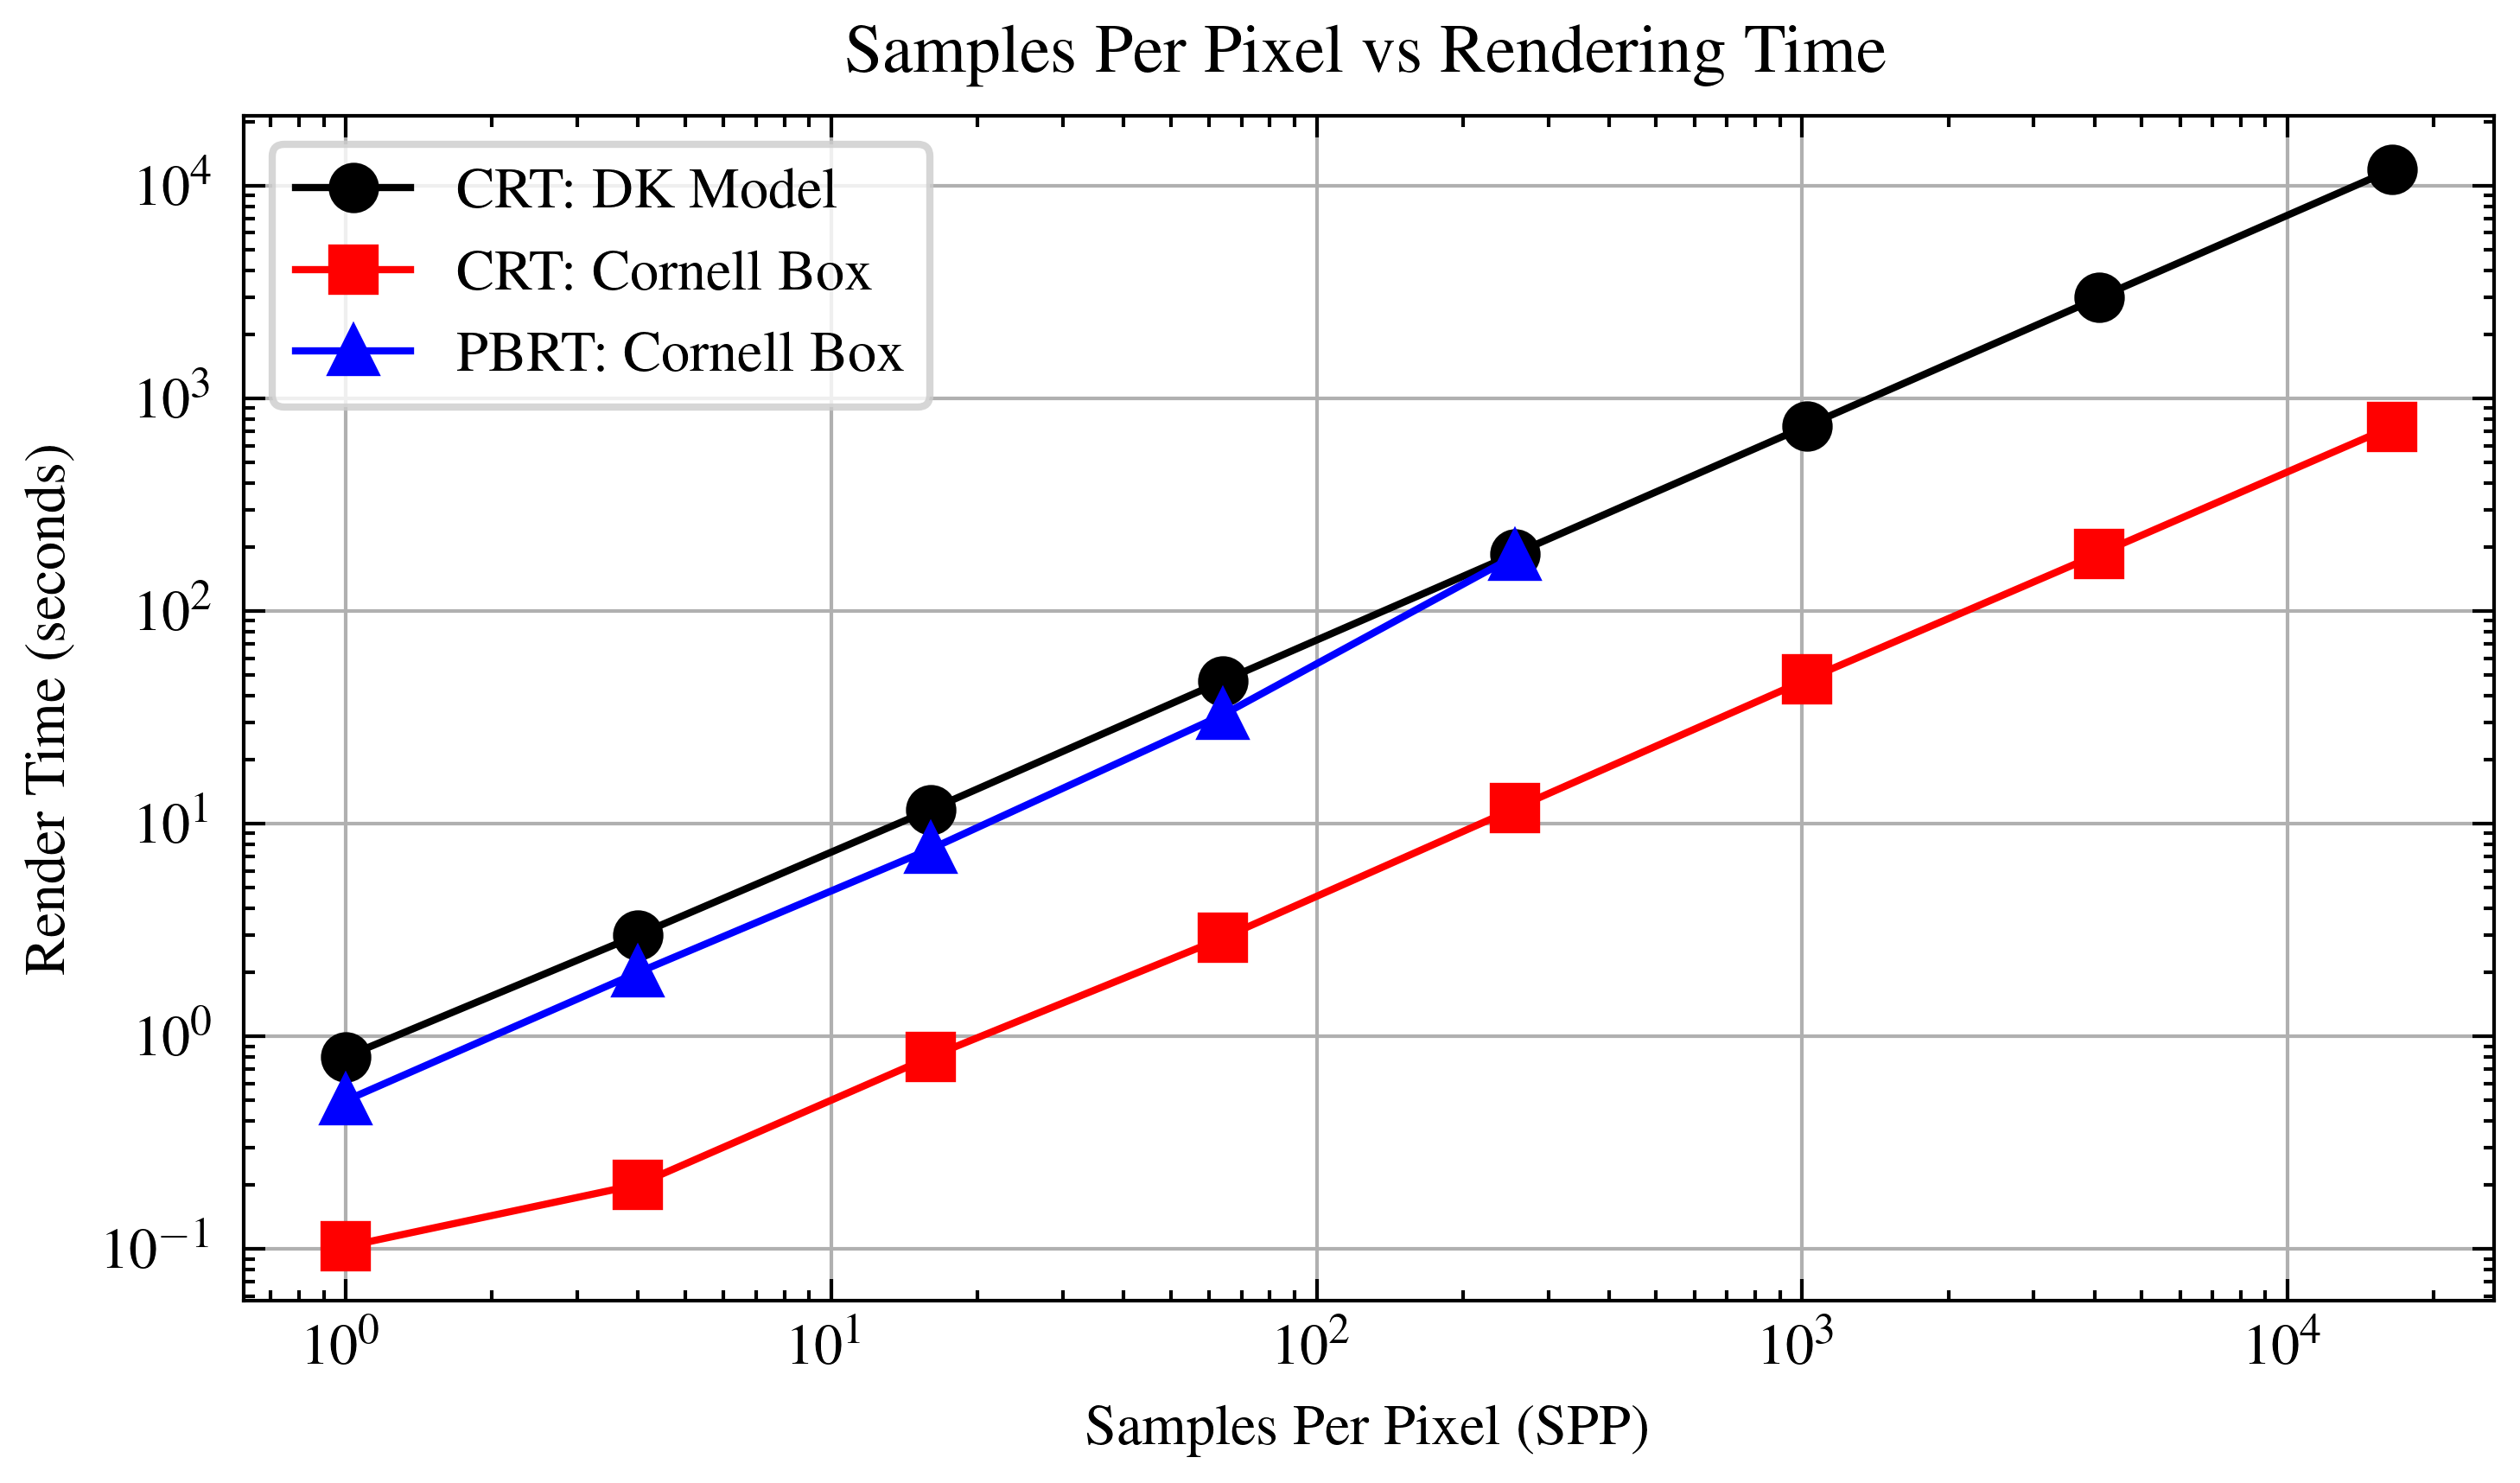
\includegraphics[width=0.45\textwidth]{render_time_vs_spp.png}
    \caption{Log-log plot of SPP vs rendering times for the CRT and PBRT CPU renderer.
    All renders have 5 max bounces and output a 1440x1440 image. The PBRT renderer
    uses the CPU \texttt{SimplePathIntegrator} and \texttt{IndependentSampler}.
    the \texttt{donkey\_kong.obj} model. The PBRT CPU renderer is run on a
    Mac Air M3 with multi-threading enabled for 8 threads.}
    \label{fig:crt_pbrt}
    \Description{CRT vs PBRT rendering time}
\end{figure}

Our CRT renderer has a 10x average speedup over the PBRT CPU renderer
for the Cornell Box test scene as shown in Figure \ref{fig:crt_pbrt}.
In a further test, doubling the dimensions of the output image to
2880x2880 resolution (or quadrupling the 
number of pixels in the image) increased the PBRT CPU rendering time from 2.0s 
14.2s compared to the CRT renderer which only increased from 0.2s to 0.8s for
a render using 4 samples per pixel. Although CRT renderer has a well define linear
scaling with the number of pixels in the image, the PBRT CPU renderer suffers greatly
from larger resolution renders despite its native multi-threading support.

% for subfile compilation
\ifSubfilesClassLoaded{%
    \nocite{*}
    \bibliographystyle{ACM-Reference-Format}%
    \bibliography{references}%
    \twocolumn
}{}
\end{document}